\section{Durchführung}
\label{sec:Durchführung}

Im folgenden Teil soll die experimentelle Untersuchung der Photoeffektes beschrieben
werden.

\subsection{Die Photozelle}
\label{sec:Die Photozelle}
Im Mittelpunkt steht hier die Photozelle, in ihr findet der Photoeffekt statt. Die
Photozelle ist ein evakuiertet Glaskolben mit zwei Elektroden. Eine davon, die
Photokathode, aus einer Metall- oder Legierungsschicht, die mit Licht bestrahlt werden
kann. Die Anode ist ein kreisförmiger Drahtring, der in einigen Milimetern Abstand
parallel zur Kathodenoberfläche angebracht ist. Der Aufbau ist in \autoref{fig:photozelle}
dargestellt.
\begin{figure}
	\centering
	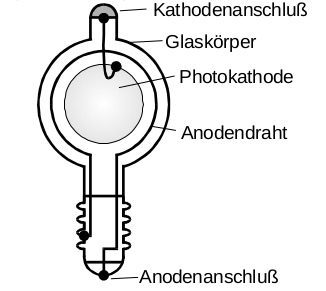
\includegraphics[height=5cm]{pictures/photozelle.png}
	\caption{Schematische Darstellung der verwendeten Photozelle \cite{anleitung}.}
	\label{fig:photozelle}
\end{figure}

Für den Versuch wird ein optischer Aufbau, wie in \autoref{fig:OptischerAufbau}
dargestellt, verwendet. Das Licht einer Spektrallampe wird gebündelt und durch ein Prisma
räumlich in die einzelnen Spektrallinien aufgeteilt. Durch den Schwankarm kann die
Spektrallinie und damit die Frequenz des Lichts ausgewählt werden, was aber immer
monochromatisch ist.

\begin{figure}
	\centering
	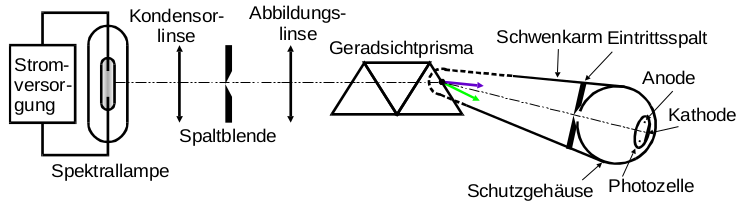
\includegraphics[height=5cm]{pictures/OptischerAufbau.png}
	\caption{Optischer Teil des Versuchsaufbaus \cite{anleitung}.}
	\label{fig:OptischerAufbau}
\end{figure}

\subsection{Energiemessung mit der Gegenfeldmethode}
\label{sec:Energiemessung mit der Gegenfeldmethode}

Um die Energie der einzelnen Photoelektronen zu bestimmen, wird hier mit der
Gegenfeldmethode gearbeitet. Dazu wird zwischen den Elektroden eine Spannung $U$ angelegt,
um ein abbremsendes Feld zu ergeugen. Der trotz jenem Feld fließende Strom zwischen Den
Elektroden wird mit einem Picoamperemeter gemessen. Der elektrische Aufbau ist in
\autoref{fig:ElektrischerAufbau} gezeigt.
\begin{figure}
	\centering
	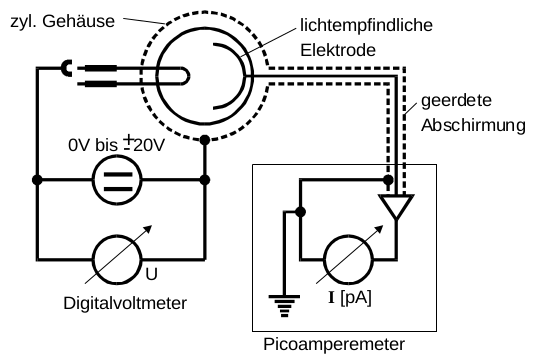
\includegraphics[height=6cm]{pictures/ElektrischerAufbau.png}
	\caption{Elektrisches Schaltbild der Messaparatur \cite{anleitung}.}
	\label{fig:ElektrischerAufbau}
\end{figure}

